\chapter{心脏增大}

心脏增大可由于心脏肥厚或(及)心脏扩张所致。

心脏肥厚主要是由于收缩期的心肌过度负荷引起,例如在心室流出道受阻时。心脏扩张主要由于舒张期心脏过度充盈引起,例如在二尖瓣或主动脉瓣关闭不全时。在多数病例中二者常同时存在或先后出现。

明显的心脏增大经胸部体格检查便可明确。但如心脏增大仅为轻度,则需经辅助检查方能证实。心脏增大可为单个心室或心房的增大,也可为普遍性或局限性增大。X线检查、超声心动图、CT扫描、核素显影、MRI能明确了解心脏各部分的增大与程度。X线胸片检查方便、费用低廉、可重复性高、人为误差小,是心脏增大的主要辅助检查方法。彩色多普勒超声血流图、多层CT、MRI能准确测量心腔大小、心室壁厚度,能对心内血流方向、速度和性质进行观察,是鉴别诊断心脏增大原因的主要手段。

心脏增大可由各种不同的疾病所致,原因复杂。见表\ref{tab16-1}。

\begin{longtable}{c}
 \caption{心脏增大疾病的分类}
 \label{tab16-1}
 \endfirsthead
 \caption[]{心脏增大疾病的分类}
 \endhead
 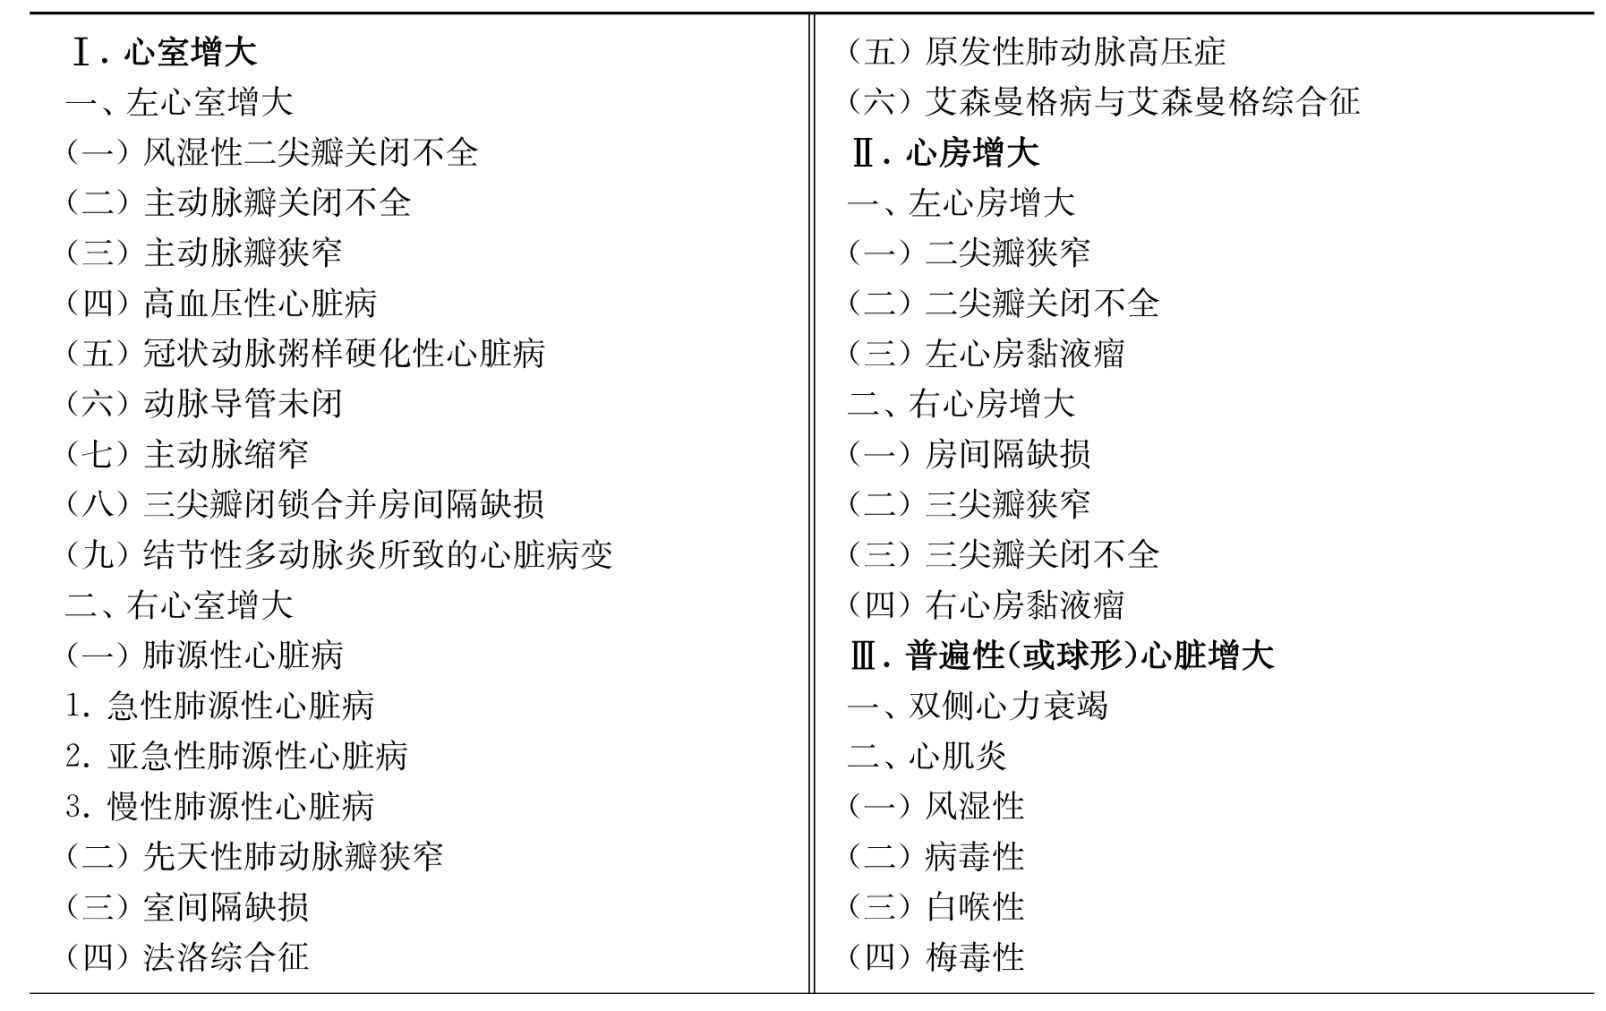
\includegraphics[width=\textwidth,height=\textheight,keepaspectratio]{./images/Image00100.jpg}\\
 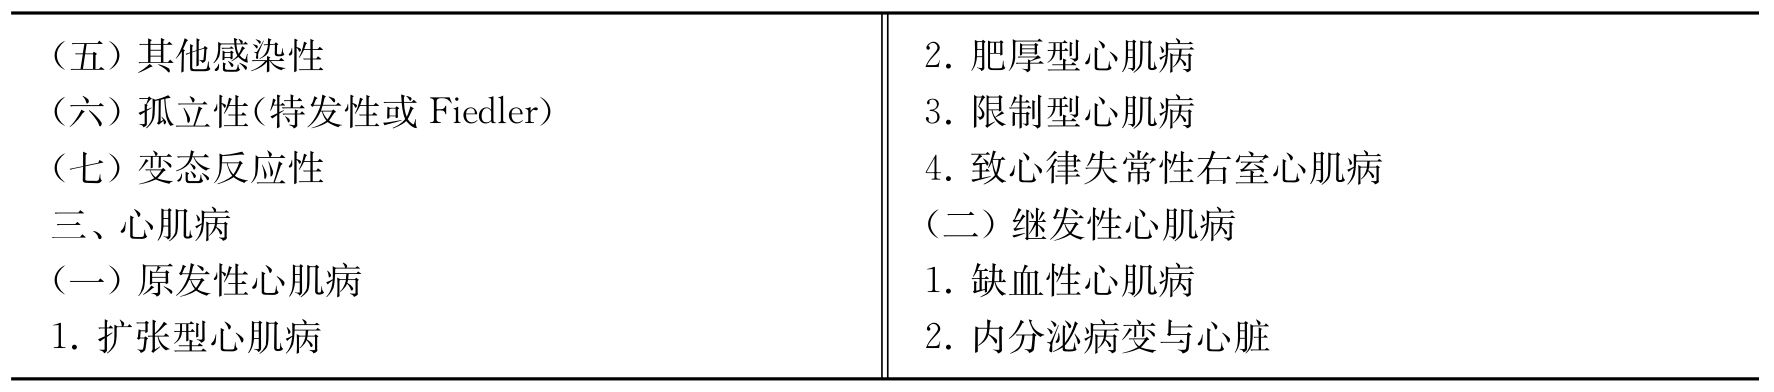
\includegraphics[width=\textwidth,height=\textheight,keepaspectratio]{./images/Image00101.jpg}
 \end{longtable}

\protect\hypertarget{text00134.html}{}{}

\section{50 心室增大}

\subsection{50.1 左心室增大}

典型的左心室增大体征包括视诊心尖搏动向左下方移位,触诊呈明显的抬举性心尖搏动,叩诊左心浊音界向左下扩大。心电图检查显示电轴左偏与左心室肥厚的征象。

\subsubsection{一、风湿性二尖瓣关闭不全}

早期仅有左室增大,心尖闻及全收缩期杂音,UCG见左室舒张末直径>50mm,左室功能失代偿后,累及左房、右心。出现左房、右室肥大及肺淤血(参见第45.1节)。

\subsubsection{二、主动脉瓣关闭不全}

左室心肌离心性肥厚,早期仅有左室舒张末期容量增加,晚期左房受累增大;胸骨右缘第2肋间及胸骨左缘3、4肋间舒张早期哈气样杂音。舒张压降低,出现周围血管征为本病主要体征(参见第45.2节)。

\subsubsection{三、主动脉瓣狭窄}

左室心肌向心性肥厚,早期即有左室肥厚,晚期失代偿时左室舒张末期容量增加。呼吸困难、心绞痛和晕厥为本病常见三联症。胸骨右缘第二肋间可闻及收缩期喷射性杂音,重要指标是跨主动脉瓣压力阶差,>30mmHg往往需要选择介入或外科治疗(参见第46节)。

\subsubsection{四、高血压性心脏病}

有长期的高血压病史,并根据体检左心室增大(心尖呈抬举性冲动,并向左下方移位)、奔马律(早期不出现)、主动脉瓣区第二音增强与金属性音调、相对性二尖瓣关闭不全所致的心尖区收缩期杂音;X线检查呈主动脉型心脏等病征。

\subsubsection{五、冠心病}

冠状动脉粥样硬化性心脏病出现心绞痛或心肌梗死时的鉴别诊断参见表\ref{tab10-3}。应当指出,当患者出现心脏增大时,排除缺血性心脏病是关键。选择性冠脉造影仍是冠心病诊断与鉴别诊断的金标准,同时行左室造影可明确左室形态与功能改变。

关于冠状动脉样硬化性心脏病的早期诊断,一般认为心电图运动负荷试验比较可靠。但在诊断时需严格掌握正确的操作技术,注意心电图的正常变异,以免导致错误的结论。另一方面,当临床可疑而心电图运动负荷试验结果阴性时,应结合全面检查结果来衡量,并作定期的复查。

心脏螺旋CT平扫可观察冠脉有无钙化,增强扫描可直接显示梗死灶,电影序列可清晰地观察室壁运动情况和准确测量心脏的舒缩功能,对室壁瘤、附壁血栓、乳头肌功能障碍和断裂等梗死后并发症有诊断价值。螺旋CT也可用于冠状动脉成像。

MRI可直接或间接显示心肌缺血和梗死灶和观察心室形态、功能变化,也可用于冠状动脉成像,并能测定冠脉血流量和血流速度,均有一定的参考价值。

\subsubsection{六、动脉导管未闭}

左心室增大兼有心底部连续性杂音,提示动脉导管未闭的诊断(参见第49.2节)。

\subsubsection{七、主动脉缩窄}

左心室增大兼有上肢血压升高、股动脉搏动减弱,提示主动脉缩窄的诊断(参见第40.3节)。

\subsubsection{八、三尖瓣闭锁合并房间隔缺损}

左心室增大伴早显性发绀,须注意三尖瓣闭锁合并房间隔缺损的可能性(参见第44.1.2节)。

\subsubsection{九、结节性多动脉炎所致的心脏病变}

本病时心脏损害常见,且主要表现为冠状动脉供血不足,冠状动脉大分支的病变可引起心绞痛,如合并血栓形成则发生心肌梗死,顽固性窦性心动过速也为常见的症状,与体温升高不相称,有人认为部分病例与迷走神经炎有关。

如病变累及肾脏,可引起高血压,而加重心脏损害的程度。

\protect\hypertarget{text00135.html}{}{}

\subsection{50.2 右心室增大}

如视诊胸骨左侧心绝对浊音区弥漫性搏动,提示右心室增大。右心室增大主要向左和向前,同时由于心脏顺钟向转位,心界仅向左扩大,而不向左下方扩大,这是与左心室增大的不同点。心电图检查显示电轴右偏与右心室肥厚的征象。X线透视时,在右前斜位较易观察到早期的右心室增大。

\subsubsection{一、肺源性心脏病}

\paragraph{(一)急性肺源性心脏病}

当体静脉或右心的栓子进入肺循环内,阻塞肺动脉或其分支有广泛的栓塞,致肺循环阻力急剧增加,超过右心室负荷的能力并使之急性扩大时,称为急性肺源性心脏病。

发病可由于体静脉或右心内血栓的脱落,外科手术伤、人工气腹术、肾周围注气等所致的空气栓塞。产科领域的羊水栓塞症等阻塞肺动脉或其广泛的分支所引起,偶尔由于蛔虫阻塞所致。

主要为肺梗塞与急性右心衰竭的征象,患者突然发生呼吸困难、胸痛、发绀、咯血。体检发现颈静脉怒张、肺动脉段浊音区增宽、胸骨左缘第2~3肋间搏动增强、收缩期与舒张期杂音、肺动脉瓣区第二音增强、三尖瓣区出现收缩期杂音。受累肺部湿性啰音、肝大与压痛,因左心输出血量剧减而发生休克,甚至引起死亡。

EDG:呈SⅠ-QⅢ图型。电轴右偏,Ⅱ、Ⅲ导联常出现肺性P波,STⅠ、Ⅱ降低,TⅠ、Ⅱ直立,STⅢ可升高,TⅢ倒置,且常有不完全性右束支传导阻滞出现,病情好转,心电图改变在较短期间恢复正常。

X线检查:可出现肺下叶卵圆形或三角形浸润阴影,重症者肺动脉段明显突出,心影增大,以及奇静脉与上腔静脉影增宽。

超声心动图:可见右室扩张,右室活动减弱,三尖瓣反流等征象。

核素显像:放射性核素肺通气灌注扫描可见栓塞处节段性灌注缺损。

选择性肺动脉造影:可显示被阻塞的肺动脉管腔狭窄或血管影中断,远端血管造影模糊而肺野相对清晰。

CT检查:螺旋CT可清楚显示肺血管内栓子。

磁共振血管成像(MRA):可示与选择性肺动脉造影相似的显像。可用于肾功能不全及(或)对碘造影剂有禁忌指征者。

血浆D二聚体测定(ELISA法):肺梗塞患者血浆D二聚体水平升高,其敏感性>90\%。但无特异性。

本病常需与急性膈面心肌梗死相区别。

\paragraph{(二)亚急性肺源性心脏病}

由癌性肺淋巴管炎引起的心脏病,被称为亚急性肺源性心脏病,国内有少数病例报告,其主要临床表现是短期内发生进行性右心衰竭,诊断主要可根据:①临床特点为患者常有剧烈的干咳、高度呼吸困难、发绀与心率加快,并于短期内死于进行性右心衰竭;②体内同时有原发性癌瘤存在,且多为腹部脏器的癌瘤(尤其是胃癌);③X线肺部平片可见有粟粒状及淋巴管炎样(网状型)阴影,是癌在肺内经淋巴道播散的征象,此病通常根据尸检而作出诊断。

\paragraph{(三)慢性肺源性心脏病}

慢性肺源性心脏病是常见的心脏病之一,通常发病于中年以上,病因较多,最常见的是由于慢性支气管炎、支气管哮喘、支气管扩张所致的慢性阻塞性肺气肿。其次是由于尘肺、广泛性肺结核病等所致的广泛性肺纤维性变合并代偿性肺气肿。较少见的是由于结缔组织疾病、原发性肺动脉高压等所致的广泛性肺小动脉梗阻,少数由于胸椎后侧凸或其他重度胸廓畸形所致的肺纤维性变、肺不张与代偿性肺气肿以及大血管扭曲等。

慢性肺源心脏病的诊断通常不难,主要的诊断根据是:①多年咳嗽或支气管哮喘病史;②体检发现呼吸困难、发绀、肺气肿体征以及不同程度的右心衰竭征象(如肝大、下肢水肿、颈静脉怒张、静脉压升高);③X线检查显示肺气肿、肺动脉段膨隆与右心室增大,心电图上有肺性P波、右心室高电压等改变;④除外其他原因所致的心脏病,临床检查如发现心窝部收缩期搏动、肺动脉瓣第二音亢进,即提示有右心室增大,在典型病例中,通常根据病史与体征,已能作出正确的临床诊断。

国内作者曾比较几种无创检查法对慢性肺源性心脏病的诊断符合率,依次为超声心动图100\%,心电图90\%,X线胸片80\%,心电向量图86\%,右心室射血分数65\%。超声心动图对右心室肥厚扩张的诊断灵敏性,优于其他检查手段,但有15\%的失检率,另外核素心血池显像、螺旋CT、MRI等均可发现右心室形态改变和功能变化。

慢性肺源性心脏病在鉴别诊断上,首先须注意鉴别者为慢性阻塞性肺气肿,当合并急性肺部感染时尤易于混淆,二者均可有慢性咳嗽、气促、桶形胸、肺部啰音、杵状指与颈静脉怒张。如临床上能证明右心室增大,则慢性肺源性心脏病可以确诊。在高度肺气肿时,由于横膈降低、心脏垂悬,X线检查有时不易肯定右心室增大,静脉压升高与臂肺循环时间延长是慢性肺源性心脏病的病征,但在重度肺气肿时静脉压也稍升高。另一方面,静脉压与臂肺循环时间接近正常时,也未能完全否定慢性肺源性心脏病的可能性,因有一部分患者由于心脏输血量增加,可使静脉压及臂肺循环时间仍在正常范围内。

慢性阻塞性肺气肿合并急性肺部感染时,临床表现虽可与慢性肺源性心脏病相似,但当感染一旦控制之后,症状迅速好转。而在慢性肺源性心脏病时,则恢复较慢而不完全。

慢性肺源性心脏病的典型心电图呈现右心室肥厚、肺性P波、电轴右移、心脏垂悬、顺钟向转位等征象,对诊断及鉴别诊断有重要意义。此外,部分患者虽无合并高血压,也可以发生左心室肥厚,而不出现典型的本病心电图改变。

此病与冠状动脉硬化性心脏病的鉴别根据是:①有慢性咳嗽或支气管哮喘病史,无心绞痛、心肌梗死的病史;②临床上以右心室增大与衰竭的征象为主,而无(或无显著的)左心室增大征象;③X线征象主要是右心室增大、肺动脉段膨隆、明显的普遍性肺气肿等;④心电图上无左心室占优势的表现;⑤杵状指的存在也为支持慢性肺源性心脏病的证据。动脉血氧饱和度测定在鉴别诊断上也有重要帮助,失代偿性肺源性心脏病不仅有动脉血氧饱和度与血氧分压的显著降低,并有明显的二氧化碳分压增高,这种情况与非肺脏疾病所致的失代偿性心脏病截然不同。

慢性肺源性心脏病患者通常是中年以上的人,常伴有周围动脉硬化,心前区可有收缩期杂音,并因动脉血氧饱和度降低、心输血量增加而可出现左心室增大,此种情况需与冠状动脉硬化性心脏病相区别,但慢性肺源性心脏病也可与冠状动脉硬化性心脏病同时并存。

\subsubsection{二、先天性肺动脉瓣狭窄}

右心室增大伴肺动脉压力减低及发绀,提示肺动脉瓣狭窄的诊断。(参见第47.1节)。

\subsubsection{三、室间隔缺损}

右心室增大伴左房、左室增大,肺充血,右室血氧含量高于右房,提示室间隔缺损诊断。(参见第46.2节)。

\subsubsection{四、法洛综合征}

法洛四联症的四项特征是:

1.室间隔缺损 常较大,位于室上嵴的后下方,累及室间隔膜部,使两心室的收缩压平衡。

2.肺动脉瓣狭窄 由于两大动脉的大小不相称或主动脉的起始部转位。

3.主动脉骑跨。

4.右心室肥厚。

法洛四联症如兼有房间隔缺损,则称为法洛五联症。

肺动脉瓣狭窄合并房间隔缺损与右心室增大,则称为法洛三联症。

法洛综合征的诊断参见第44.1.2节。

\subsubsection{五、原发性肺动脉高压症}

右心室增大伴肺动脉压增高,肺血流减少,提示原发性肺动脉高压症(参见第44.1.1节)。

\subsubsection{六、艾森曼格病与艾森曼格综合征}

艾森曼格病是指大的高位室间隔缺损合并主动脉右位、肺动脉高压与分流方向颠倒,而无肺动脉瓣狭窄,艾森曼格综合征是指左右心之间任何一种缺损,如房间隔缺损、室间隔缺损或动脉导管未闭,合并肺动脉高压和肺血管阻力增高,伴有分流方向颠倒(参见第44.1.2节)。

\protect\hypertarget{text00136.html}{}{}

\section{51 心房增大}

\subsection{51.1 左心房增大}

左心房明显增大时,心脏叩诊可发现左第三肋间相对浊音界增宽。轻度或中度左心房增大则在X线透视右前斜位观察下最为清楚,吞钡检查可见增大的左心房压迫食管,使之向后移位,左心房呈弧形向后突出。心电图P波时程延长或出现典型的双峰P波,称为“二尖瓣型P波”。

\subsubsection{一、二尖瓣狭窄}

左心房增大伴肺淤血、心尖区舒张期中晚期隆隆样杂音提示二尖瓣狭窄诊断(参见第45.2节)。

\subsubsection{二、二尖瓣关闭不全}

左心房增大伴左心室增大、肺淤血、心尖区收缩期吹风样杂音提示二尖瓣关闭不全诊断(参见第45.1节)。

\subsubsection{三、左心房黏液瘤}

左心房增大伴非劳力性呼吸困难,心尖闻及舒张和收缩期杂音及肿瘤扑落音、广泛全身反应(发热、恶病质、体循环和肺循环栓塞等)提示左心房黏液瘤可能,超声心动图有较高诊断价值(参见第45.2节)。

\subsection{51.2 右心房增大}

右心房明显增大时,叩诊右侧心界增宽,但不如X线检查的清楚。在前后位透视下,右心房几乎构成右心缘的全部轮廓,仅靠近膈的一小段是右心室。

\subsubsection{一、房间隔缺损}

右心房增大伴肺淤血,右心室增大,右房血氧含量高于上腔静脉提示左向右分流房间隔缺损(参见第47.1节)。

\subsubsection{二、三尖瓣狭窄}

右心房增大伴体循环淤血,右心室缩小,三尖瓣听诊区闻及舒张期杂音提示三尖瓣狭窄(参见第48.2节)。

\subsubsection{三、三尖瓣关闭不全}

右心房增大伴右室增大,三尖瓣听诊区闻及收缩期杂音提示三尖瓣关闭不全(参见第48.1节)。

\subsubsection{四、右心房黏液瘤}

右心房增大伴体循环淤血、发绀,三尖瓣听诊区闻及舒张期杂音及肿瘤扑落音提示右心房黏液瘤可能,超声心动图有较高诊断价值(参见第48.2节)。

\protect\hypertarget{text00137.html}{}{}

\section{52 普遍性(或球形)心脏增大}

普遍性心脏增大可见于许多心脏病。首先需与心包积液相鉴别(参见表\ref{tab17-2})。

\subsection{52.1 双侧心力衰竭}

当左心衰竭引起肺阻性充血与肺动脉高压,同时导致右侧心力衰竭时,则产生双侧心力衰竭的临床表现,心界向左右两侧扩大。

\protect\hypertarget{text00138.html}{}{}

\subsection{52.2 心肌炎}

重症心肌炎常有下列的临床表现:①心尖搏动弥散与移位;②心脏普遍性增大;③心搏增快(也可因重度房室传导阻滞而显著减慢,心音减弱,心律不齐,心尖收缩期杂音,有时也出现舒张期杂音);④奔马律;⑤心电图异常。

心肌炎主要有下列几种:

\subsubsection{一、风湿性心肌炎}

风湿性心肌炎无特殊的症状与体征,可有体温升高、心搏加快、血沉加快、C反应蛋白试验阳性、白细胞增多等,只表示风湿热处于活动期。其他症状如心前区疼痛、心脏迅速增大、心音减弱、心搏加快等,需与合并心包炎鉴别。心尖部收缩期杂音,可能由于心肌损害、心脏迅速增大所致,但需与风湿性心内膜炎鉴别。奔马律是合并心肌炎相当可靠的体征,但不常出现。

心律失常与心电图改变可能为心肌损害的主要佐证,甚至可能为心肌损害的唯一证据,心电图改变以P-R间期延长为多见,具有诊断意义。其他常见心电图改变包括频发性多源性期前收缩、二联律、心房扑动或纤颤,由于心电图改变有时不固定或持续时间甚短,故在疑似病例应在不同时期反复进行心电图描记对比,甚至多次Holter检查方能发现较有诊断意义的改变。

超声心动图对风湿性心肌炎有一定的诊断价值,风湿性心肌炎患者可见瓣膜增厚(二尖瓣最常见)、瓣膜脱垂和二尖瓣腱索断裂、瓣膜反流和房室腔增大。另有报道瓣膜上可发现回声均匀的小结节,抗风湿治疗后所有结节消失,提示可能是病理学检查所见的风湿性疣状赘生物。

\subsubsection{二、病毒性心肌炎}

目前已证实能引起心肌炎的病毒有:小核糖核酸病毒,如柯萨奇病毒、埃可病毒、脊髓灰质炎病毒等;虫媒病毒,如登革热病毒、流行性出血热病毒、黄热病毒等;腺病毒;流感病毒;副黏病毒,如流行性腮腺炎病毒、麻疹病毒、呼吸道合胞病毒等;疱疹病毒,如单纯疱疹病毒、水痘-带状疱疹病毒、巨细胞病毒;风疹病毒;狂犬病毒;肝炎病毒;呼吸道肠道病毒;脑心肌病毒;淋巴细胞脉络丛脑膜炎病毒等。其中以柯萨奇病毒、埃可病毒、流感病毒、流行性腮腺炎病毒和脊髓灰质炎病毒最常见。

病毒性心肌炎临床表现差异性很大,大多数患者呈亚临床型,可以完全没有症状,有症状者轻重不一。多有心悸、气促、心前区不适,重者可并发心律失常、心力衰竭、心源性休克等。累及心包及(或)胸膜者可出现剧烈胸痛。半数患者其病前1~3周有前驱感染史。

主要体征为心界扩大、心动过速、各种心律失常(期前收缩多见),心尖可闻及收缩期杂音,重症者可出现奔马律和交替脉。

血清学检查:①白细胞可轻度增高;②ESR可增快;③心肌酶可增高。

病毒学检查:①发病早期,采取患者的咽部涂拭物、血液、粪便、心包积液等能分离出病毒,有助于本病的诊断;②补体结合、病毒中和抗体和血凝抑制试验等也有诊断价值,在病程第2、3周后,血清补体效价如增高4倍以上,即有诊断意义。

ECG:对本病诊断敏感性高,但特异性低,以心律失常尤其是期前收缩最常见,其中室性期前收缩占80\%。另可见房室传导阻滞、ST-T改变、心室肥大、Q-T间期延长、低电压等改变。

X线检查及超声心动图:两者改变均无特异性,可有心脏增大,搏动减弱有时可见心包积液,超声心动图可有左室收缩或舒张功能障碍,有时可见附壁血栓。

核素显影:\textsuperscript{99m}
TC-MIBI心肌显像表现为心肌弥散性分布小灶性或局灶性核素灌注稀疏,提示心肌坏死,晚期未受累心肌细胞代偿性肥大时,也可见局限性核素浓集灶。67GA显像表现为炎症受累心肌异常放射性浓集区,心血池显像可见心脏扩大,室壁运动减弱,左右心EF、最大排空率和充盈率均下降。

磁共振成像(MRI):可见受损心肌异常高信号表现,同时可指引心肌活检取样,提高活检阳性率,也可评估心脏收缩舒张功能改变。

心内膜心肌活检:对诊断病毒性心肌炎颇有价值,可检出病毒、病毒基因片段或病毒蛋白抗原,但阴性结果不能排除本病。

\paragraph{诊断和鉴别诊断}

国内成人病毒性心肌炎诊断标准如下:

\subparagraph{1.病史与体征}

在上呼吸道感染、腹泻等病毒感染后3周内出现心脏表现,如出现不能用一般原因解释的感染后重度乏力、胸闷、头昏(心排血量降低所致)、心尖第一心音明显减弱、舒张期奔马律、心包摩擦音、心脏扩大、充血性心力衰竭或阿-斯综合征等。

\subparagraph{2.上述感染后3周内新出现下列心律失常或心电图改变:}

(1)窦性心动过速、房室传导阻滞、窦房阻滞或束支阻滞。

(2)多源、成对室性期前收缩,自主性房性或交界性心动过速,阵发或非阵发性室性心动过速,心房或心室扑动或颤动。

(3)两个以上导联ST段呈水平型或下斜型下移≥0.01mV,或ST段异常抬高,或出现异常Q波。

\subparagraph{3.心肌损伤的参考指标}

病程中血清心肌肌钙蛋白Ⅰ或肌钙蛋白T(强调定量测定)、CKMB明显增高。超声心动图示心腔扩大或室壁活动异常及(或)核素心功能检查证实左室收缩或舒张功能减弱。

\subparagraph{4.病原学依据}

(1)在急性期从心内膜、心肌、心包或心包穿刺液中检测出病毒、病毒基因片段或病毒蛋白抗原。

(2)病毒抗体:第二份血清中同型病毒抗体(如柯萨奇B组病毒中和抗体或流行性感冒病毒血凝抑制抗体等)滴度较第一份血清升高4倍(2份血清应相隔2周以上),或一次抗体效价≥640者为阳性,320者为可疑阳性(如以1∶32为基础者则宜以≥256为阳性,128为可疑阳性,根据不同实验室标准作决定)。

(3)病毒特异性:IGM以≥1∶320者为阳性(按各实验室诊断标准,需在严格质控条件下),如同时有血中肠道病毒核酸阳性者更支持有近期病毒感染,对同时具有上述“1”、“2”[(1)、(2)、(3)中任何一项]、“3”中任何二项,在排除其他原因心肌疾病后,临床上可诊断急性病毒性心肌炎;如同时具有“4”中(1)者,可从病原学上确诊急性病毒性心肌炎;如仅具有“4”中(2)、(3)者,在病原学上只能拟诊为急性病毒性心肌炎。

如患者有阿-斯综合征发作、充血性心力衰竭伴或不伴心肌梗死样心电图改变、心源性休克、急性肾衰竭、持续性室性心动过速伴低血压或心肌心包炎等一项或多项表现,可诊断为重症病毒性心肌炎。如ECG示ST段抬高并有心肌酶升高,需注意与急性心梗鉴别。

病毒性心肌炎有时需与β受体反应亢进症相鉴别,后者多为青壮年女性,主诉心悸、胸闷、头昏、心动过速等症状,心电图显示窦性心动过速,可有ST-T改变与期前收缩,易被误诊为病毒性心肌炎。精神因素常为发病诱因,而与病毒感染无关,患者尚有较明显的易激动、失眠、多汗等交感神经兴奋症状,也可有微热,血压可偏高,血沉、抗“O”、甲状腺吸131碘试验、结核菌素试验等均正常。心脏不增大,用普萘洛尔类药物治疗有特效,口服普萘洛尔治疗后,心电图出现心率减慢,ST-T改变也恢复正常。

病毒性心肌炎还需与风湿性心肌炎相鉴别,下列情况支持病毒性心肌炎而不支持风湿性心肌炎的诊断:前者抗“O”效价不增高,血沉通常仅轻度或中等度加快,血象白细胞总数大多减少或正常(少数增多),多有相对性淋巴细胞增多,并可发现异形淋巴细胞。病毒学检查更有重要鉴别诊断意义。

\subsubsection{三、白喉性心肌炎}

白喉并发心肌炎者较常见,但临床诊断颇多困难,只根据临床检查,必有颇多漏诊。在病程中不同时期反复作心电图检查,可能提高确诊率。患者在恢复期间仍有心率加快或明显减慢,或其他心律失常,提示并发心肌炎的高度可能性。

\subsubsection{四、梅毒性心肌炎}

病理解剖上可区分为弥漫性与局限性两型。此病大多数侵犯左心室心肌,尤其是室间隔部,临床上以心脏普遍性增大、进行性心力衰竭为主要征象。此病需注意与脚气病性心脏病等相区别,如患者有梅毒感染史,而无维生素B\textsubscript{1}
缺乏史与多发性神经炎,血清康、华氏反应阳性,则支持梅毒性心肌炎的诊断,又如同时出现左束支传导阻滞心电图,则梅毒性心肌炎可能性更大。

\subsubsection{五、其他感染性心肌炎}

由于猩红热、大叶性肺炎、伤寒、急性细菌性痢疾、立克次体感染、弓形体病、军团菌病等所致的心肌炎,程度通常较轻,但偶尔也可相当严重。如患者在病程或恢复期间出现显著的心动过速或其他心律失常,提示并发心肌炎的可能性。

\subsubsection{六、孤立性心肌炎}

孤立性心肌炎也称特发性或Fiedler心肌炎,是罕见而原因未明的心脏病。此病可发生于任何年龄,但以年轻成人为多见,经过大多为急性,少数为亚急性与慢性。患者多有以心脏扩大为主的心脏增大,并常有心室壁血栓形成的特征性表现,但不并发心包炎与心内膜炎。患者主要表现为呼吸困难、发绀、衰弱与心前区痛,发热也常见,可并发肺与脑栓塞。

体检常发现心脏增大,并往往出现奔马律、心律失常与交替脉等。血沉正常或加快,心电图无特征性改变,常显示左心室损害的征象,病情有每况愈下的趋势,经过通常为数周,主要因进行性心力衰竭而死亡。

此病需与急性型克山病相区别,但发病地区不同。又需与脚气病性心脏病相区别,但患者无维生素B\textsubscript{1}
缺乏史。国内报告的一组尸检5例中,3例为暴死者,于发病25分钟至4小时内死亡,一向身体健康的年轻成人,有类似急性心肌梗死的表现而暴死者,应考虑此病的可能性。

\subsubsection{七、变态反应性心肌炎}

约半数血清病所致的变态反应性心肌炎病情较重,因出现心电图改变而需住院治疗。

文献曾报道有些药物可引起变态反应性心肌炎,但少见,且都发生于过敏性体质的人。此类药物有磺胺类、青霉素、金霉素、链霉素、保泰松、氯丙嗪、牛痘疫苗等。

心电图表现为ST段与T波异常等改变,病理改变主要是嗜酸性粒细胞性间质性心肌炎。

\protect\hypertarget{text00139.html}{}{}

\subsection{52.3 心肌病}

心肌病是泛指一组主要发生于心脏肌肉层的病变,主要表现为心脏增大,最后发生。心力衰竭,1980年世界卫生组织与国际心脏病学联合会划分此病为两大类:①原发性心肌病(原因未明的);②特异性(继发性)心肌病。

虽然这些疾病原发地损害心肌,但常累及心内膜、心包,甚至心瓣膜,心肌病从此分为原发性与继发性两类,原发性心肌病一般单独侵犯心脏,与继发性心肌病不同,后者的心脏是受全身性疾病所累及,病变侵及其他器官,下文分别讨论原发性与继发性心肌病的诊断与鉴别诊断。

\subsubsection{一、原发性心肌病}

\paragraph{(一)扩张型(充血型)原发性心肌病(DCM)}

男性罹患较多,发病多在20~50岁之间。本型心肌病病因未明,病毒感染、免疫机制缺陷、遗传因素、血管活性物质和微血管痉挛、心肌超微结构和生化代谢改变、易感因素(营养不良、酗酒、高血压、妊娠等)等受到注意。病理改变为四个心腔均增大并扩张,心室扩张甚于心房,并伴有不同程度的心肌肥厚,心腔内可出现血栓。

临床表现为充血性心力衰竭征象,以气促和水肿最常见。部分患者以体循环栓塞或肺栓塞为首发症状,主要体征为心脏扩大,心率快,常有心律不齐,并可闻及病理性S3、S4,心率快时构成奔马律。

ECG:可见各种类型的室性与房性心律失常、ST-T改变及病理性Q波。

X线检查:示心影增大,心胸比>0.6,晚期心影呈球形,心脏搏动普遍性减弱,伴不同程度的肺充血,有时伴胸腔积液。克山病亦属扩张型心肌病范畴。

超声心动图:常示以下几项特点:①“一大”:全心腔扩大,尤以左心室扩大为显著,左室舒张期末内径>50~55mm,或≥2.7cm/m\textsuperscript{2}
;②“二薄”:室壁、室间隔变薄,<7~11mm;③“三弱”:室壁及室间隔运动普遍性减弱;④“四小”:瓣膜口开放幅度小,并可测定左心室射血分数(LVEF)与舒张功能、肺动脉高压,也可显示心腔内附壁血栓。

核素显影:核素心血池显像可见心脏扩大,室壁运动普遍性减弱,整体射血分数及各节段局部射血分数均下降。心肌灌注显像则见多节段性花斑状改变或节段性减低,心肌代谢显像极少有代谢缺损,多数表现为代谢不均匀,灌注/代谢异常的心肌节段匹配者占多数。

磁共振成像(MRI):可见受累心腔扩大,相应心房心室收缩功能减弱。另磁共振光谱分析(MRS)可测定心肌代谢功能障碍。

螺旋CT:能准确测量心脏径线,对心功能进行定量分析,观察室间隔和室壁运动情况,并可进行冠状动脉平扫以鉴别缺血性心肌病。

心导管和血管造影检查:左室舒张末压、左房压及肺毛细血管楔压升高,心排出量和每搏量减少,射血分数降低。左室造影可见左室腔扩大,左室壁运动减弱,冠脉造影常正常。

心内膜心肌活检:缺乏特异性。

血清学检查:近年来有报道血清中抗心肌肽类抗体,如抗心肌线粒体ADP/ATP载体抗体、抗肌球蛋白抗体、抗β1受体抗体、抗M2胆碱能受体抗体阳性,也有助于作为DCM的辅助诊断方法,并与DCM心力衰竭的严重程度相关。

诊断和鉴别诊断

国内诊断标准如下:①临床表现为心脏扩大、心室收缩功能减低,伴或不伴有充血性心力衰竭和心律失常,可发生栓塞和猝死等并发症。②心脏扩大:X线检查心胸比>0.5;超声心动图示全心扩大,尤以左心室扩大为显著,左室舒张期末内径≥2.7cm/m\textsuperscript{2}
,心脏可呈球形。③心室收缩功能减低:超声心动图检测室壁运动弥漫性减弱,左室射血分数小于正常值。④必须排除其他特异性(继发性)心肌病和地方性心肌病(如克山病),方可做出本病的诊断。

心脏增大需与心包积液相鉴别,可借助于超声检查。1/3病例有心尖部收缩期杂音,需与风湿性二尖瓣关闭不全相区别(参见第45.1节)。心肌硬化型冠状动脉硬化性心脏病的心脏可显著增大,如伴有乳头肌功能不全,心尖部可出现收缩期杂音,如兼有心电图ST-T改变,可与充血型原发性心肌病相似。但原发性心肌病发病常在40岁以前,无高血压动脉硬化的表现,治疗后充血性心力衰竭消失、心影缩小,均支持原发性心肌病的诊断。慢性心肌炎也有心脏普遍性增大、心律失常、舒张早期奔马律等表现,与原发性心肌病相似,国外文献也有报道病毒感染引起充血型心肌病,诊断主要根据病史、病毒分离与抗体滴定度测定的结果,如心肌炎为风湿性,则可参考过去风湿热与全心炎的病史,以及有关的实验室检查结果而确定之。

本病需与克山病鉴别:克山病病因未明,硒缺乏和营养因素受到重视,流行病学特点为:①分布于我国东北至西南走向的从黑龙江至云南的一条狭长地带内;②病区主要分布于丘陵山区;③在高发年与低发年的差异;④在北方主要侵犯育龄期妇女,南方多见于断奶后、学龄前儿童,但性别无差异;⑤外来人口在病区居住3个月以上方能发病。

本病近年修订的分型是:

\subparagraph{1.急性型}

起病急,也可由潜在型或慢型发展而来,有心源性休克、肺水肿等急性心功能不全的表现,此型心脏扩大多不明显,但心律失常多见而易变,伴重度心律失常者为重症病例。

\subparagraph{2.慢性型}

发病慢,往往在不知不觉中发病,也可由其他三型演变而来,心脏中度或明显增大,心功能Ⅱ~Ⅲ级,主要表现为慢性充血性心力衰竭(参见第92节)。

\subparagraph{3.亚急性型}

发病稍慢于急型,多在症状出现后一周左右发生心源性休克或(及)充血性心力衰竭,多发生于断奶后和学龄前儿童,患儿较常有栓塞性并发症。

\subparagraph{4.潜在型}

患者通常无明显自觉症状,心功能Ⅰ级,无急、慢或亚急性型病史,或心电图上有ST-T改变、QT时间延长者,称不稳定的潜在型。

克山病的诊断主要根据:①患者是地方病区居民,并除外其他原因的心脏病(但需注意可能合并存在);②患者有头晕、胸闷、恶心、呕吐、心悸、气短、全身乏力等症状;③体检发现心界扩大、心尖区常有Ⅰ~Ⅱ级吹风样收缩期杂音、第一心音低沉或同时第二心音减弱、心律失常、血压低下、脉搏细弱等;④心电图出现各型房室或束支传导阻滞或其他心肌损害征象;⑤X线检查心脏向两侧扩大,尤以左心室为著,搏动减弱或不规则,或有局部僵直区等。若患者具备第①、②项,再具备③、④、⑤项中任何一项,即可诊断为本病。在急性型或慢性型(痨型)急性发作时,常先有谷草转氨酶活性升高,往往为早期病征之一。

有人指出患者脉搏触诊常有颇多特点,如脉率不稳定、忽快忽慢、过缓或过速、沉细微弱、左右强弱不等、脉律不整、轻度运动后变为沉细微弱或出现交替脉、重脉等。对临床诊断甚有帮助,临床医生如能熟练掌握症状、心音听诊与脉搏触诊三者,即可作为早期诊断潜在型和急性型克山病的主要手段。又如掌握肝大和肝颈静脉回流征,就可帮助痨型克山病的早期诊断。

克山病需与Fiedler心肌炎、风湿性心肌炎、脚气病性心脏病、结缔组织疾病所致心肌病、感染性心肌炎等相鉴别。脚气病性心脏病通常发生于炎热季节,右心室增大较为明显,心律大多规则,有多发性神经炎的表现,维生素B\textsubscript{1}
治疗有特效。风湿性心肌炎有链球菌感染史、发热、多发性关节炎、心脏杂音、白细胞增多、血沉高度加快、皮下结节或环形红斑等表现,有助于互相区别。

\paragraph{(二)肥厚型(梗阻性)原发性心肌病}

本病常为常染色体显性遗传疾病,偶尔为获得性,以心肌非对称性肥厚,心室腔变小为病理特征,心肌肥厚主要累及左心室、室间隔,亦可累及右心室,偶见同心性心肌肥厚。左心室容量正常或缩小,而左心室舒张压常增高,流出道前后出现压力阶差。过去本病也有称为特发性肥厚性主动脉瓣下狭窄、原发性肥厚性阻塞性心肌病、特发性心肌肥厚等。

心尖肥厚型心肌病(AHCM)是HCM中的变异型,心肌肥厚局限在左室乳头肌以下的心尖部位,流出道前后无压力阶差。

临床表现及分型:HCM按血流动力学可分为两型:心脏收缩时引起左室流出道梗阻者称“梗阻性肥厚型心肌病”。不引起梗阻者称“非梗阻性肥厚型心肌病”。肥厚型心肌病患者的晕厥和胸痛(可呈心绞痛发作)是最有特征性的症状,多在30岁之前出现,劳力性呼吸困难亦常见。猝死常由心律失常导致,通常引人注意的第一个体征是颈动脉异常搏动,颈动脉搏动的上升支快速而短促,与正常者不同。常有心前区抬举性心尖搏动。心浊音界向左、右两侧扩大,部分病例左侧扩大。大多数病例在胸骨左缘第三、四肋间听到Ⅱ~Ⅲ级收缩期喷射性杂音,或伴有震颤,常可听到第四心音。

ECG:典型改变为左心室肥厚劳损与深的异常Q波,ST-T改变及房室、束支传导阻滞也较常见。

心音图:于胸骨左缘第三、四肋间可录出收缩中、晚期高频菱形杂音。患者吸入亚硝酸异戊酯后,收缩期杂音振幅增大,心率加快。下蹲体位或注射普萘洛尔后则振幅减低。

X线检查:心脏轻度增大,以左室为主,左房也可扩大。

超声心动图:①左心室肥厚,常表现为不对称性室间隔肥厚,典型者≥15mm,舒张期室间隔的厚度与后壁之比>1.3;②左心室流出道狭窄,一般<20mm;③流出道有压力阶差者,二尖瓣前叶出现异常的收缩期前向运动(SAM),并可见二尖瓣反流;④左室腔变小,室间隔运动减弱;⑤主动脉瓣在收缩期呈半开放状态;⑥心室舒张功能障碍,但处于高动力状态,LVEF常>0.7。

核素显影:核素心血池显像示不对称性心肌肥厚及局部室壁活动异常,左心室容积减低,左室游离壁活动增强,LVEF增高,舒张功能障碍。心肌代谢显像显示HCM患者心肌肥厚部位心肌组织存在代谢障碍。另有报道心肌灌注显像示部分HCM患者有节段性灌注缺损,提示心肌缺血可能。

磁共振成像(MRI):①室间隔或(及)室壁肌局限性或普遍性肥厚,收缩末期厚度>15mm,与其同层面左室后壁或正常心肌厚度比值≥1.5;②肥厚室间隔和室壁肌与正常心肌MRI信号相同;③肥厚肌块向左室腔内凸出,致室腔缩小、变形或(及)流出道狭窄;④肥厚心肌收缩期增厚率下降(△T<30\%);⑤心室舒张期充盈速率减慢和达到充盈峰值的时间缩短。

螺旋CT:可见室间隔或(及)室壁肌局限性或普遍性肥厚、室腔不大或缩小,可伴有流出道狭窄。并可测定心肌肌块重量、心肌收缩率和增厚率。

心导管和血管造影检查:左室舒张末压升高,有梗阻者左室腔与流出道之间压差>20mm,左室造影显示左室腔缩小变形,呈香蕉状或舌状,也可呈“芭蕾舞足征”。冠脉造影示肌桥比率较高,冠状动脉内径较粗大,以左冠动脉增粗为主。

心内膜心肌活检:心肌细胞排列紊乱,畸形肥大,免疫荧光测定法示肥厚心肌内儿茶酚胺含量增高。

心尖肥厚型心肌病(AHCM)

此型心肌病是HCM中的变异型,心肌肥厚局限在左室乳头肌以下的心尖部位,流出道前后无压力阶差。它在临床表现、心电图、超声心动图等诸方面有特殊临床特点。AHCM中以男性为多,活动后心前区胸闷、压榨样疼痛为主要症状,也可见心悸、气促等症状。

心电图具有以下特点:①ST段下移:以V\textsubscript{2~5}
最常见;②T波对称性深倒置,以胸导V\textsubscript{3~5}
为主,呈TV\textsubscript{4} ≥TV\textsubscript{5} >TV\textsubscript{3}
的改变关系;③R波振幅增高,以胸导改变为主,呈RV\textsubscript{4}
≥RV\textsubscript{5} >RV\textsubscript{3} 的规律变化;④无Q波形成。

超声心动图检查表现为左心室近心尖部位的间隔和左室后壁肥厚,而室间隔中上部无增厚。核素心肌显像显示心尖部位的心肌肥厚,呈斑点状心肌血流分布异常。磁共振检查显示心尖部心肌肥厚,冠状动脉造影多正常,左心室造影显示左室舒张期末心尖部肌肉肥厚,可呈“黑桃形”改变。据有关文献报道,有无“黑桃形”改变与心尖部肌肉的局部非对称有关。

鉴别诊断心尖肥厚型心肌病常因心电图胸导联ST-T改变而被误诊为急性冠脉综合征,本病还需与高血压心脏病、室间隔缺损、主动脉瓣狭窄、二尖瓣关闭不全相鉴别。

\paragraph{(三)限制型(闭塞型)原发性心肌病(RCM)}

病因未明,可能与病毒感染、营养不良、自身免疫等多种因素有关,病理学改变是心肌浸润性及纤维化病变、心内膜纤维化(伴有或不伴有嗜酸性粒细胞增多)。

临床表现及分型:RCM按WHO建议分以下两种类型:

\subparagraph{1.心内膜心肌纤维化(EMF)}

本病多见于热带非洲,散发性病例见于各处。特征是广泛的心内膜和心内膜下纤维组织增生,心室腔被致密的纤维组织部分地闭塞,纤维组织上可形成致密的白色而厚的被覆物,纤维组织可将乳头肌和腱索固定于心室后壁,产生明显的二尖瓣关闭不全。

\subparagraph{2.嗜酸性粒细胞增多性心内膜心肌病}

也称勒夫勒(Löffler)心内膜炎和纤维弹力组织性心内膜炎,是嗜酸性粒细胞增多症的一种亚型,以心脏受累为主要表现。在任何一侧心室均可以形成大块附壁血栓,使心室腔减小,并可引起肺栓塞和体循环栓塞。常伴有肝脾大和其他脏器嗜酸性粒细胞浸润的临床表现。本病病理特点为心内膜增厚,弹力纤维增生,嗜酸性粒细胞浸润,心肌纤维化等。

临床症状以充血性心衰为主,可出现充血性心衰的各种体征。

ECG:低电压、束支传导阻滞、ST-T改变等。

X线检查:心脏轻度增大,伴心房扩大时呈球形,少数患者有心内膜钙化影。

超声心动图:①心腔狭小,心尖多闭塞;②心内膜层超声反射增强提示增厚;③室壁运动减弱;④心室舒张早期充盈快,中、晚期极慢;⑤可见二尖瓣、三尖瓣反流。

核素显影:核素心血池显像示心房增大,心室舒张、收缩功能均降低。

磁共振成像(MRI):①心房显著扩大,自旋回波脉冲序列示心房内大量缓慢血流所致中~高信号;②心室流入道缩短、变形,心尖闭塞或圆隆,流出道扩张;③室壁增厚,以心内膜为主,内膜面凹凸不平,可见极低信号(提示钙化灶);④室壁运动减弱;⑤梯度回波电影MRI示房室瓣反流;⑥可显示有无心包增厚及(或)胸腔积液等。

螺旋CT:可见心房扩大、心室腔变小,流入道缩短,心尖部闭塞,心室心内膜增厚,室壁运动减弱等征象。

心导管和血管造影检查:心室内压力曲线示舒张功能严重受损,舒张早期心室压力常不能降至零,房室瓣开放后室内压迅速升高,然后呈平台样(“平方根”征)。心脏造影可见流入道及心尖部心腔狭小甚至闭塞,流出道扩张。

心内膜心肌活检:勒夫勒心内膜炎确诊常靠心内膜心肌活检,但活检结果并非总是阳性,EMF时活检对诊断可有帮助。

鉴别诊断

本病特别需与缩窄性心包炎鉴别,CT及MRI可清楚显示有无心包增厚,对鉴别两病有较高价值。

\paragraph{(四)致心律失常性右室心肌病(ARVC)}

本病为常染色体显性遗传病伴不完全外显,感染、自体免疫因素和凋亡亦受到注意。ARVC的病理解剖学特征是心室肌被脂肪纤维组织替代,可以仅累及右室心肌局部,也可弥漫整个心室。但最常发生于右室心尖部、漏斗部及膈面或下壁,即所谓“发育不良三角”,室间隔很少受累,右心室常增大。

临床上表现可以无症状,或有心悸、轻度头晕、运动相关的晕厥甚至猝死。室性心动过速常见,另可见室上性心动过速、房颤、房扑、完全房室传导阻滞、尖端扭转性室性心动过速等。

ECG:①常规心电图:ARVC患者室速发作时呈左束支传导阻滞图形且电轴多左偏,局限于右室流出道的ARVC发生室速时电轴也可右偏,但比较少见。窦性心律时的心电图检查约70\%的患者有不正常表现,主要有右胸导联(V\textsubscript{1~3}
),特别是V\textsubscript{2} 导联T波倒置,V\textsubscript{1}
导联QRS波群时间延长>110毫秒。部分患者呈完全或不完全右束支传导阻滞图形,30\%的ARVC患者能在右胸导联特别是V\textsubscript{1}
导联上见到QRS波终末、ST段起始部有小棘波,称epsilon波。②运动心电图:对于临床症状不典型的患者可作运动心电图,50\%患者可诱发出室性心律失常,但运动试验阴性不能排除ARVC。有报道对ARVC患者进行运动心电图检查,发现可诱发ST段抬高>0.1mV,且这些患者冠脉造影均正常,这也提供了一种对于隐匿性ARVC患者无创性的筛查方法,但必须排除冠脉疾病。③信号平均心电图:各文献报道ARVC患者晚电位阳性率不等,但均在80\%以上,且与猝死率相关。但如果ARVC患者病灶非常局限,即使有室速发作,信号平均心电图检测结果也可能正常。

超声心动图:①右心室扩大,右心室与左心室收缩末期直径比>0.5,但若为局限病变可无此表现;②右心室受累部位(单个或多个),表现为室壁的低动力或无运动状态;③右心室局部膨隆或囊状突出;④孤立性右室流出道扩张;⑤右心室舒张期结构变形,肌小梁排列紊乱及右心室节制带(moderate
band)或调节束异常。

核素显影:①放射性核素心血池扫描可见右室扩大、局部膨隆、射血分数下降等形态及功能异常;②核素心肌灌注显像能显示出右室心肌内局部缺损区,揭示ARVC患者心肌受损情况。

磁共振成像(MRI):早期ARVC患者经超声等检查很难发现,但磁共振检查可较清晰地显示室壁变薄或局部增厚。另可见右室肌小梁排列紊乱、右室局部膨出、右室室壁瘤样变,并可根据信号回声不同,将心室肌内微小病态的纤维脂肪组织与正常沉积脂肪组织相区分,有助于判断病灶与室速的起源部位,并指导心内电生理进行定位标测。

\subparagraph{心导管和血管造影检查}

\hypertarget{text00139.htmlux5cux23CHP16-3-3-1-4-1-1}{}
1.右室造影

①右室舒张末期容量增加伴室壁运动弥漫性减弱;②左侧位右室后壁造影剂滞留;③右室流出道在舒张期局限性膨出及收缩期运动障碍;④右室发育不良三角出现局限性运动障碍;⑤右室前壁心尖部节制带远端有横置肥厚的肌小梁被裂沟分隔。其中第5条对ARVC有高度特异性,由于右室形态结构上的复杂性使造影检查有一定局限性,不可能发现小而局限的病灶,故造影阴性不能排除ARVC。

\hypertarget{text00139.htmlux5cux23CHP16-3-3-1-4-1-2}{}
2.左室造影

20\%~50\%的患者存在左室节段运动异常,容积增加,EF下降,部分患者可见到二尖瓣脱垂和左室环状运动低下带。

\hypertarget{text00139.htmlux5cux23CHP16-3-3-1-4-1-3}{}
3.心内膜心肌活检

对于临床上可疑患者,心内膜心肌活检有助诊断,通常标本取自室间隔及右室游离壁,阳性所见为正常心肌组织被纤维脂肪组织所替代。

\hypertarget{text00139.htmlux5cux23CHP16-3-3-1-4-1-4}{}
4.心内电生理研究

心内电生理研究及程序电刺激可以检测心律失常的发生机制、形态特征、诱发与终止条件以及对心律失常起源病灶精确定位,心内电生理检查的结果可以指导进行药物治疗、ICD植入及射频消融治疗。

\subparagraph{诊断标准}

目前,国际上工作组普遍应用ARVC的Task
Force诊断标准。诊断ARVC需包含2个主要条件,或1个主要条件+2个次要条件,或不同组别的4个次要条件,金标准为心内膜活检或外科手术的组织病理学检测结果。

ARVC的Task Force诊断标准:

\hypertarget{text00139.htmlux5cux23CHP16-3-3-1-4-2-1}{}
1.全部/局部功能下降及结构改变

(1)主要条件:

1)严重的右室扩张及EF下降(无或仅轻度左室受累)。

2)右室壁局部瘤样膨出。

3)严重右室局部扩张。

(2)次要条件:

1)轻度的右室扩张及EF下降,无左室受累。

2)轻度右室局部扩张,局限右室活动低下。

\hypertarget{text00139.htmlux5cux23CHP16-3-3-1-4-2-2}{}
2.室壁组织特征

心内膜活检见心肌被纤维脂肪组织替代。

\hypertarget{text00139.htmlux5cux23CHP16-3-3-1-4-2-3}{}
3.复极异常

次要条件:大于12岁成人平时ECG见右心前V\textsubscript{2}
、V\textsubscript{3} 导联T波倒置,右束支阻滞图形。

\hypertarget{text00139.htmlux5cux23CHP16-3-3-1-4-2-4}{}
4.除极传导异常

(1)主要条件:右心前ECGV1~3导联QRS波延长>110毫秒,可见epsilon波。

(2)次要条件:SAECG,晚电位阳性。

\hypertarget{text00139.htmlux5cux23CHP16-3-3-1-4-2-5}{}
5.心律失常

主要条件:ECG、Holter、运动试验可见持续或非持续的左束支阻滞图形室速,频发室性期前收缩>1000/24h。

\hypertarget{text00139.htmlux5cux23CHP16-3-3-1-4-2-6}{}
6.家族史

(1)主要条件:家族中患者经心肌活检或外科证实ARVC。

(2)次要条件:家族中小于35岁患者由于右室发育不良导致猝死。

\subsubsection{二、继发性心肌病}

\paragraph{(一)缺血性心肌病}

是指心肌缺血引起的,以心肌纤维化为主的心肌病。基本病因是冠心病,常有多次及(或)多发性心肌梗死史,心肌变性、坏死和纤维瘢痕形成,导致心肌收缩力减退和心室顺应性下降,最终发展为心衰。若心衰反复发作,心脏普遍性扩大,酷似扩张型心肌病改变,少数类似限制型心肌病。

临床表现:有明确冠心病史,以心绞痛和心衰症状为主,心脏呈普大型,左室扩大为主,左室扩大合并相对性二尖瓣关闭不全以及合并乳头肌功能不全时,心尖部可闻及收缩期杂音。

ECG:可有病理性Q波、ST-T改变和各种心律失常。

X线检查:心脏普遍增大,以左室扩大为主,心脏搏动减弱和肺淤血征象。

超声心动图:①心脏普遍性扩大,以左室为主,并有舒张末期内径增大;②室壁运动节段性减弱;③收缩前期(PEP)延长,左室射血时间(LVET)缩短,PEP/LVET比例增加,左室射血分数(LVEF)下降,常<0.35。

核素显影:核素心血池显像可见心腔扩大,室壁运动节段减弱,左心功能不全,心肌灌注显像呈按冠状动脉分布的多节段性灌注缺损。心肌代谢显像可见心肌代谢缺损,且多数有心肌灌注/代谢不匹配。

螺旋CT:平扫可见冠脉内钙化,电影可见心脏增大,室壁运动节段性减弱等征象。

心导管和血管造影检查:左室舒张末压、左房压和肺动脉楔压增高。左室射血分数降低,左室腔扩大和多节段、多区域室壁运动障碍。冠脉造影常示多支冠脉病变。

鉴别诊断

本病需特别与原发性扩张型心肌病相鉴别,核素显影、冠脉造影和螺旋CT等检查有较高价值。

\paragraph{(二)内分泌病变与心脏}

\subparagraph{1.甲状腺功能亢进性心脏病}

甲状腺功能亢进症以20~40岁为最多,而并发心脏病者多在40岁以上,女性占多数。血液循环时间正常或加快。在严重心力衰竭出现之前,静脉压常为正常。有人相信甲状腺功能亢进症状不少为充血性心力衰竭的单独的原因,且多见于女性,随年龄与病程而递增。并发心房纤颤者发生心力衰竭也比无心房纤颤者为多。甲状腺功能亢进性心脏病的诊断可根据下列条件:

(1)已确诊为甲状腺功能亢进症。

(2)患者有下列心脏病病征之一项或多项:①心脏增大;②心律失常,如心房纤颤、传导阻滞等,但仅有窦性心动过速或期前收缩者不计入内;③心力衰竭。

(3)除外其他原因的心脏病。

(4)治疗甲状腺功能亢进症奏效后,心脏病基本治愈。

另外,遇到下列情况也应考虑甲状腺功能亢进性心脏病的可能:①原因不明的阵发性或持久性房颤,心室率不易控制者;②无法解释的持续性窦性心动过速;③心力衰竭用常规治疗收效不大者;④已有器质性心脏病的患者,伴发甲状腺功能亢进症状,而洋地黄疗效较差者。

心力衰竭时可使基础代谢率升高,故不能单独根据基础代谢率测定来确定诊断,必须结合甲状腺功能亢进的其他临床表现、血清蛋白结合碘测定或放射性核素131碘试验,以协助诊断。

甲状腺功能亢进性心脏病患者大多可在心尖区听到收缩期杂音,其响度可达Ⅲ级,有时也可出现舒张期杂音。心尖搏动弥散于心前区,触诊有如震颤,不少病例伴有心房纤颤,患者又以女性为多,可被误诊为风湿性二尖瓣膜病。所不同者,此种舒张期杂音如果存在,也仅为轻度,并非隆隆样,控制甲状腺功能亢进后,上述异常体征均可消失。此外也无左心房增大的征象。

老年甲亢心脏病患者的甲亢症状和体征常常缺如或不典型,患者常以心悸、胸闷气短、心绞痛就诊,易与冠状动脉硬化性心脏病相混淆,需仔细鉴别。在甲状腺功能亢进性心脏病时,心绞痛可能由于代谢过高、心动过速、心肌负荷过度,致心肌相对缺氧所致,故其出现与甲状腺功能亢进的严重程度有密切关系。甲状腺功能亢进被控制之后,心绞痛即消失。

此外,少数病例可伴有血压升高,收缩压偶尔可达180mmHg,可与高血压性心脏病相混淆。所不同者,此病时舒张压不升高,反而降低,脉压增大,故不难与高血压性心脏病相区别。

\subparagraph{2.甲状腺功能减退性心脏病}

是比较少见的疾病,又称黏液性水肿心脏病。甲减时,进行性黏液性水肿可引起心脏增大,可由心肌扩张及肥大或心包积液所致。

甲状腺功能减退性心脏病主要表现是:①有甲减的典型表现,如体重增加、畏寒、嗜睡等;②在黏液性水肿的基础上,出现劳动后呼吸困难或端坐呼吸、心绞痛、心动过缓等。

甲状腺功能减退性心脏病的诊断可根据下列的条件:

(1)确诊甲减。

(2)心动过缓,心脏扩大及(或)心包积液等心脏病征。

(3)除外其他原因的心脏病。

(4)经甲状腺激素治疗后,上述变化好转。

黏液性水肿患者的全身性水肿、浆膜腔积液、体重增加、呼吸困难、心悸、心脏增大、心音减弱、异常的静脉压,均可与充血性心力衰竭相似,两者难以鉴别。

黏液性水肿与黏液性水肿并发充血性心力衰竭的鉴别诊断要点是:①黏液性水肿的静脉压往往正常而血压减低。并发充血性心力衰竭时,则静脉压及血容量却明显增高。②黏液性水肿时肺动脉压及右心室压力正常,活动后心输出量增加,但无肺动脉或全身性静脉压的增高,这种情况在并发充血性心力衰竭时相反。③胸部X线检查,黏液性水肿时可有心脏增大及大量浆膜腔积液,但无肺充血的征象,并发充血性心力衰竭时则肺充血是其特征。④黏液性水肿的皮下水肿及积液对洋地黄及利尿剂治疗无反应,需要给予甲状腺激素替代治疗才能减轻水肿及积液。并发充血性心力衰竭时,则洋地黄有疗效。

\subparagraph{3.肢端肥大症性心肌病}

部分肢端肥大症患者无高血压和冠心病,但出现不能用其他原因解释的心力衰竭、心律失常,应考虑肢端肥大症性心肌病的可能。本病无特征性病理改变。ECG常示电轴左偏,ST段压低,T波低平或倒置和束支传导阻滞。超声心动图可见室间隔非对称性肥厚或左室肥厚,易被误诊为原发性肥厚型心肌病。实验室检查可见血浆生长激素及血浆生长介素C升高。头颅CT和脑部X线检查可确定垂体病变部位。

\subparagraph{4.糖尿病性心肌病}

糖尿病患者如无冠脉病变或瓣膜病变,但有明显的心绞痛或急性心肌梗死的临床表现,伴有心脏扩大、心律失常及(或)心力衰竭,且排除其他原因的器质性心脏病,应考虑糖尿病性心肌病可能。其特征性病理改变为广泛的心肌微血管病变,心肌变性、退行性变和广泛局灶性坏死及心肌纤维化。可有各种心律失常。超声心动图可见心室顺应性降低,舒张功能障碍,晚期可有收缩功能障碍,EF降低,搏出量减少等。

\paragraph{(三)酒精性心肌病}

是指长期饮烈性酒致使心肌变性,表现为心脏扩大、心功能不全的一种心肌病。中年男性多见,其临床表现及实验室器械检查结果均酷似原发性扩张型心肌病。但其心肌活检示磷酸肌酸激酶、乳酸脱氢酶、苹果酸脱氢酶等升高。本病诊断主要依靠患者长期饮酒史,实验室器械检查示心脏增大和戒酒及治疗后心脏可缩小,再饮酒后复发。

\paragraph{(四)围产期心肌病(PPCM)}

是指发生在妊娠最后3个月或产后6个月内原因不明的心肌疾病,临床表现与DCM相似,(参见第40.3节)。

\paragraph{(五)药物性心肌病}

是指由于服用某些药物的患者,因药物对心肌的毒性作用,引起心肌损害所导致的心肌疾病。其临床表现和实验室器械检查结果与原发性扩张型心肌病、肥厚型(梗阻性)原发性心肌病相似。临床上能致心肌损害的药物众多,最常见的包括:①抗癌药物如阿霉素、柔红霉素等;②抗精神病药物如氯丙嗪、奋乃静等;③三环类抗抑郁药如氯丙咪嗪、阿米替林等;④可卡因。本病诊断主要依靠患者服药史,服药前无心脏病证据,服药后出现心律失常、心脏增大、心功能不全等征象,且无法用其他心脏病解释。

\paragraph{(六)心动过速性心肌病(tachycardia-induced cardiomyopathy)}

是指由室上性或室性快速性心律失常引致的进行性心肌病变和心力衰竭。可单独发生或与其他心脏疾病合并发生。本病病因未明,心肌能量代谢障碍和心脏交感神经系统改变受到关注。本病主要临床表现为快速性心律失常伴心室增大、心室收缩功能受损及心力衰竭。实验室器械检查结果与原发性扩张型心肌病相似,控制心动过速后,心功能可有改善。

心动过缓,心脏舒张期越长,回心血量越多,心腔可能越大,严重心动过缓,需要植入心脏永久起搏器的患者常有心脏增大,尤其是心腔扩大。

\paragraph{(七)贫血性心脏病}

重度慢性贫血常引起心脏扩张、心肌肥厚与变性,临床上出现心绞痛发作甚至心力衰竭。病因最多为钩虫病,患者皮肤与黏膜显著苍白,常有下肢凹陷性水肿而无发绀。由于周围血管扩张,舒张压降低,脉压增大,可出现周围血管征。心脏叩诊发现普遍性增大,心尖区与心底部可听到功能性收缩期杂音。由于心脏扩张,有时可在心尖区、主动脉瓣区与肺动脉瓣区听到功能性舒张期杂音。静脉压正常,臂舌与臂肺循环时间反而见缩短。心电图显示窦性心动过速、T波平坦或倒置、ST段降低、低电压等改变。

贫血性心脏病的诊断主要依据:①患者有重度慢性贫血;②有上述的心血管病征;③除外其他原因的心脏病;④经抗贫血治疗奏效后,上述的心脏病征基本复原。

\paragraph{(八)系统性红斑狼疮性心脏病}

系统性红斑狼疮累及心脏者并非少见,且可引起心脏增大、心包积液甚至充血性心力衰竭。其临床表现可与风湿热、亚急性细菌性心内膜炎相似,但病理改变截然不同。心内膜、心包膜与心肌都可累及,病理解剖所见为心内膜下胶原纤维肿胀、弥漫性或局限性心肌炎症、冠状动脉分支内壁损害与血栓形成等。临床症状主要为发热、关节痛、贫血、心动过速、心尖区收缩期杂音(偶尔可出现舒张期杂音)、心包积液征、奔马律、非特异性心电图改变。如不及时积极治疗,往往死于充血性心力衰竭。

心脏病变发生于系统性红斑狼疮基础之上,如对此病有所警惕,则不致漏诊,但需注意与亚急性细菌性心内膜炎、风湿热等相区别。

\paragraph{(九)系统性硬皮病所致的心脏病变}

硬皮病少见。心脏受累通常为此病的晚期现象。主要症状是劳动后气促与心律失常,偶尔引起心包炎,心脏损害通常并不严重,引起心力衰竭者也少见。但一旦发生心力衰竭,对洋地黄治疗反应不佳。

\hypertarget{text00139.htmlux5cux23CHP16-3-3-2-10}{}
(十)脚气病性心脏病

是一种严重的脚气病类型,多见于热带与亚热带,较多侵犯从事强度体力劳动的青壮年人,或妊娠期和哺乳期的妇女。尤其是在炎热的季节,当食物中维生素B\textsubscript{1}
有长期的缺乏,而患者又罹患急性传染病或胃肠功能紊乱时,较易罹患。

脚气病性心脏病的主要临床表现是:胸闷、心悸、气促、发绀、尿少(但无蛋白尿)、颈静脉怒张搏动、心脏普遍性增大(尤以右侧心显著)、心动过速、心尖区收缩期杂音、收缩压升高、舒张压降低、脉压增大、周围血管征等。偶尔发生严重的心律失常。其他维生素B\textsubscript{1}
缺乏症状如纳差、膝腱反射消失、步态失调等也出现。急性心力衰竭常迅速发生,患者病情沉重、面容憔悴、发绀、端坐呼吸、烦躁不安,如不及时救治,往往迅速死亡。

脚气病性心脏病是心肌与神经系统的联合性病变,本病甚少发生,仅有少数病例报道,有人曾提出本病的诊断标准可供参考:

1.心脏增大而心律多正常(窦性):正常心律起源于窦房结,故患者虽发生奔马律,也为正常心律。

2.下垂性水肿。

3.静脉压升高。

4.周围神经炎或糙皮病。

5.非特异性心电图改变 一般只有低电压、T\textsubscript{Ⅰ}
倒置、QRS\textsubscript{Ⅰ} 轻度改变、Q-T间期延长等。

6.有心脏病病变而能除外其他原因。

7.显著的营养缺乏超过3个月以上。

8.经维生素B\textsubscript{1} 治疗后症状缓解,心脏病病征消退。

\hypertarget{text00139.htmlux5cux23CHP16-3-3-2-11}{}
(十一)高山性心脏病变

是高山病[高山(原)适应不全症]的表现之一。高山病是机体对高山环境一个反应过程,同时也是一个病理的过程。人由海拔较低、气压较高的地区,进驻海拔较高、气压较低的高山或高原地区(国内报告在1167m以上,或1433m以上),如未经适应锻炼,则可因缺氧而引起的一系列的病理现象,有人对高山病曾作出以下的临床分型(表\ref{tab16-2})。

\begin{table}[htbp]
\centering
\caption{高山病的临床分型}
\label{tab16-2}
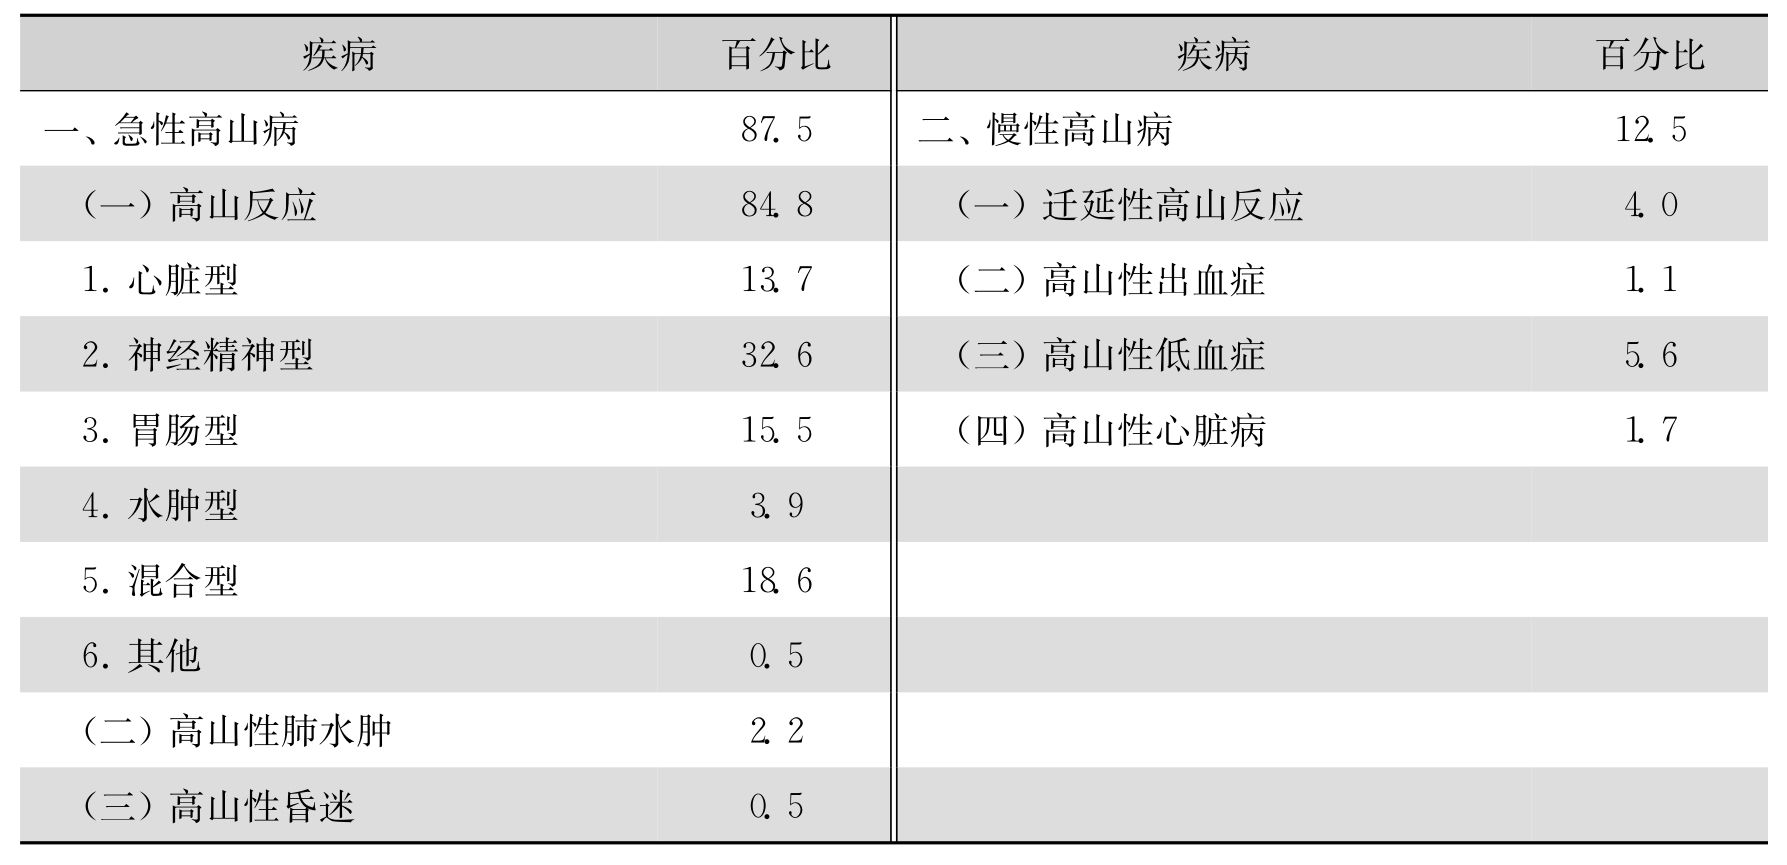
\includegraphics[width=5.94792in,height=2.875in]{./images/Image00102.jpg}
\end{table}

高山病所致的心脏病变,起病急慢不等,因此可区分为下列两种类型:

\hypertarget{text00139.htmlux5cux23CHP16-3-3-2-11-1}{}
1.急性高山性心脏病

发生于进入高山(高原)后的半年内,是心脏对缺氧环境的一种急性反应。患者出现心悸、气短、心率加快等心脏症状,并伴有血中红细胞增多与血红蛋白量增加。心音多数亢进,心底部第二音常有分裂,多数出现心脏杂音,心脏扩大、心律不齐可出现,少数发展为急性左心衰竭。

\hypertarget{text00139.htmlux5cux23CHP16-3-3-2-11-2}{}
2.慢性高山性心脏病

发生于进入高山(高原)后的半年后,是因患者在高原地区工作一段时期之后,未能适应缺氧环境而引起的一种心脏病。患者主诉心慌、心前区不适与气喘。体检发现患者可有明显的发绀,心脏呈球形增大、心尖区与三尖瓣区收缩期杂音、肺动脉瓣第二音亢进。大多数有全身性水肿及其他体循环淤血征象。此病需除外其他原因所致的心脏病而确定之,特别是脚气病性心脏病与高血压性心脏病。

高山性心脏病的主要诊断依据为:①原发病,发病在海拔3000m以上;②肺动脉高压表现;③排除其他心肺疾病;④患者迁居平原地区后症状缓解或消失。

\hypertarget{text00139.htmlux5cux23CHP16-3-3-2-12}{}
(十二)心脏淀粉样变性

心脏淀粉样变性十分少见,可为原发性或继发性,而以后者较多。二者的鉴别有重要意义,因如发现病因,除去病因后可治愈此病。

凡患者在40岁以上,有病因未明的心脏增大与心力衰竭,或伴有肺功能不全,应考虑原发性淀粉样变性的可能性。如兼有巨舌症,则可能性更大。如在慢性化脓性疾病过程中,出现明显的蛋白尿或肾病综合征,或兼有原因明确的心脏增大与心力衰竭,则有继发性淀粉样变性的可能性。

心脏淀粉样变性可表现为限制型或充血型心肌病的临床病象。充血性心力衰竭引起呼吸困难、水肿、颈静脉怒张、奔马律、胸水与腹水,心房纤颤常见。偶尔引起心绞痛,并可出现类似陈旧性心肌梗死的心电图。传导阻滞可引起晕厥。淀粉样变性累及肺脏时可引起慢性肺源性心脏病。肾脏虽常累及,但高血压不常见。

突出的心电图表现是低电压,尤其是肢体导联,左心室导联可有T波倒置,常有P-R间期延长与束支传导阻滞。常有心律不齐,例如期前收缩与心房纤颤。心电图可出现陈旧性心肌梗死。

X线检查心脏可呈不同程度的普遍性增大,但心脏轮廓在透视下可显示“刻板样”,搏动高度减弱。

超声的典型表现为二维超声上可见增厚的左心室游离壁及间隔呈颗粒闪光点回声。

原发性约半数病例出现巨舌症,有重要的提示诊断价值。心脏淀粉样变性的诊断只有根据活体组织检查,牙龈活检或肝、脾穿刺活检也有诊断价值,但后者有一定的危险。刚果红试验在诊断上可供参考,但无危险性。

近年国内一组心脏淀粉样变性5例报告,本病临床表现无特异性,轻者无症状。重者表现为心律失常、传导障碍、难治性心力衰竭。本病又是多系统病变,症状广泛,水肿、贫血、蛋白尿、肝脾大、巨舌症及胃肠功能障碍等均可出现。超声心动图可发现心脏受累严重程度、病情演变和预后,但确诊主要依靠活组织病理学检查。

\hypertarget{text00139.htmlux5cux23CHP16-3-3-2-13}{}
(十三)放射性心肌病

胸部或纵隔恶性肿瘤放疗时,心脏受到放射线损伤可引起放射性心脏病。包括心包炎、心肌病、冠脉病变、瓣膜病变和传导系统病变。放射性心肌病常与心包炎和冠脉病变同时出现,心肌弥漫性或片状纤维化,临床表现、实验室检查与原发性心肌病相似。

\hypertarget{text00139.htmlux5cux23CHP16-3-3-2-14}{}
(十四)浸润性心肌病

是指某些异常代谢产物在心肌内积聚或浸润而引起的伴有心室舒张功能减弱的限制性心肌病,收缩功能也可同时受损,本类疾病常具有遗传性。常见的有:

\hypertarget{text00139.htmlux5cux23CHP16-3-3-2-14-1}{}
1.Fabry病

为X-连锁糖鞘脂代谢异常的隐性遗传病。心肌组织的溶酶体内糖脂贮积是本病多种心血管表现的原因。典型心脏表现包括心绞痛和心肌梗死(但冠脉造影正常)、左室壁增厚、左室功能不全和二尖瓣反流。ECG示房室传导阻滞、P-R间期缩短、ST-T改变等。超声心动图示左室壁厚度增加,状若HCM。

\hypertarget{text00139.htmlux5cux23CHP16-3-3-2-14-2}{}
2.血色素沉着病

为铁沉积于各种实质性器官所致。心脏受累的结果可导致混合性的扩张型/限制型心肌病。

\hypertarget{text00139.htmlux5cux23CHP16-3-3-2-14-3}{}
3.糖原贮积症

本病成年患者可出现心脏受累情况,最常见的标志是在ECG和超声心动图上呈现明显的左室肥厚征象。

\protect\hypertarget{text00140.html}{}{}

\subsection{52.4 爱泼斯坦畸形}

如心影呈球形增大,肺野清朗,而肺动脉段凹陷,心电图P波高大,右束支传导阻滞,则很可能是爱泼斯坦畸形。患者常有发绀,右至左分流通过未闭的卵圆孔或房间隔缺损。本病常易被误诊为心包积液(参见第44.1.2节)。

\protect\hypertarget{text00141.html}{}{}

\subsection{52.5 大血管错位}

在完全性大血管错位时,后前位X线检查心影呈“横置的蛋形”,因双侧心室增大,主要是右心室增大所致,后前位显示大血管根部特别狭窄,而侧位观察大血管根部明显增宽(参见第44.1.2节)。

\protect\hypertarget{text00142.html}{}{}

\section{53 局限性心脏增大}

局限性心脏增大只有经X线检查方能作出诊断。

\subsection{一、心包囊肿与心包憩室}

为先天性疾病,多数患者无自觉症状,X线检查见心包膜近膈角如发现有明显阴影,尤其在右侧者,应高度怀疑本病可能。参见第27.4节。

\subsection{二、心室壁瘤(心脏膨胀瘤)}

心室壁瘤比较少见,通常在心肌梗死后形成,最多位于左室心尖部。急性心肌梗死之后出现顽固性心力衰竭,或反复的心绞痛发作,或栓塞现象,均须考虑心室壁瘤形成。高血压是促进心室壁瘤形成的一个重要因素。由于心室壁的瘤样膨出,心界多呈局限性扩大,心脏搏动也较弥散。听诊心音减弱,有时有收缩期杂音。

X线检查是诊断心室壁瘤的重要依据,其特点为:①左心缘局限性凸出,或呈不对称性扩大;②多轴透视检查可见凸出部心缘的搏动减弱、消失或反相搏动;③局部阴影密度增加或偶见钙化现象;④病变部位有心包粘连现象等。记波摄片上可详细观察到左心室各部分的搏动改变。

MRI更能清楚地显示室壁瘤的图形。核素心血池扫描示心影突出部分与心腔相连。左室造影可显示室壁瘤的部位、大小和瘤体内有无血栓形成,同时能反映出心动周期左心室容积变化。心电图上有广泛心肌梗死的征象和ST段持久升高,超声检查也有助于诊断。

心室壁瘤最常见的临床表现是反复发作的心力衰竭,主要死亡原因是严重的心律失常(心室纤颤、三度房室传导阻滞等)、心力衰竭、栓塞症等。

\subsection{三、心脏肿瘤}

心脏肿瘤临床上少见,可为原发性和继发性,后者较前者多见。超声心动图、MRI、螺旋CT对其诊断有较高价值,尤其是螺旋CT在超声心动图难以诊断的潜在性肿瘤的诊断及肺部、纵隔和胸腔并发病变的观察方面,有明显优势。

\subsubsection{(一)原发性心脏肿瘤}

80\%为良性,多能手术治疗。

原发性良性心脏肿瘤多为黏液瘤,其中3/4位于左心房,左心房黏液瘤的诊断参见第45.2节。

原发性恶性心脏肿瘤(几乎都是肉瘤)甚少见,下列情况提示此病的可能性:①迅速发展的心脏方面的自觉症状与心律失常;②迅速发展的心脏增大或心脏部分性增大,在记波图上显示僵硬的、轮廓改变的心脏外形;③血性心包积液,抽液后迅速再行渗聚;④病程短(平均4~6个月),超声检查有助于发现较大的心脏肿瘤。

心脏肉瘤以血管肉瘤多见。患者多为中青年人,肿瘤侵及心包脏层则出现大量血性积液或心包压塞。诊断价值以MRI、经食管二维超声心动图(2DE)、经胸2DE最高。确诊有赖于活检组织病理学检查。心包积液中肿瘤细胞检出率低。

\subsubsection{(二)继发性心脏肿瘤}

远较原发性为多见。原发肿瘤一般为癌,多位于肺、纵隔、胃、卵巢、肝、乳腺等器官及组织,尤以肺及纵隔更常见。

此病主要表现为心力衰竭、心律失常或心包积液,凡原因未明的、未能用洋地黄控制的进行性心力衰竭,原因未明的严重心律失常或穿刺抽液后迅速重再渗聚的血性心包积液,均须考虑恶性心脏肿瘤的可能性,特别是40岁以上的患者。如发现原发肿瘤的存在,则大致可能定心脏肿瘤为继发性。

X线检查常显示下列的改变:①心脏外形不整或局限性扩张;②心脏内阴影增浓(心肌浸润),搏动减弱或暂停;③迅速的心影增大或块质形成。结合临床表现与超声检查,可能确定此病的临床诊断。本病预后恶劣,易发生猝死。

\protect\hypertarget{text00143.html}{}{}

\section{参考文献}

1.中华医学会心血管病学分会.急性心力衰竭诊断和治疗指南.中华心血管病杂志,2010,38(3):195-208

2.中华医学会心血管病学分会.慢性心力衰竭诊断治疗指南.中华心血管病杂志,2012,40(2)

3.袁家讷,等.运动201铊心肌断层显像对冠心病的诊断价值.中华心血管病杂志,1989,17:271

4.汪公亮,等.关于慢性肺源性心脏病合并冠心病的诊断标准.天津医药,1980,8:19

5.郑更生,等.心房黏液瘤的诊断.中华内科杂志,1978,17:344

6.全国心肌炎心肌病专题座谈会纪要.中华内科杂志,1987,26:597

7.中华医学会儿科学分会心血管学组.病毒性心肌炎诊断标准(修订草案).中华儿科杂志,2000,38(2):75

8.心肌炎心肌病对策专题组.关于成人急性病毒性心肌炎诊断参考标准和采纳世界卫生组织及国际心脏病学会联合会工作组关于心肌病定义和分类的意见.中华心血管病杂志,1999,27:405-407

9.陈璘,等.核素显像在病毒性心肌炎诊疗中的意义.中华内科杂志,2000,39(11):749-750

10.苏诚钦,等.成人柯萨奇A9型病毒感染心肌炎.中华医学杂志,1980,60(6):345

11.陈昌生,等.成人病毒性心肌炎暴发性流行15例临床分析(摘要).中华医学杂志,1980,60(6):336

12.孙明,等.病毒性心肌炎40例临床观察.中华内科杂志,1979,18:415

13.钱维顺,等.肠道病毒性心肌炎------附10例分析.中华内科杂志,1981,20(1):19

14.张国培,等.心肌树胶样肿两例报告.中华内科杂志,1959,7:164

15.江顺林,等.伤寒、副伤寒心肌炎的诊断.中华内科杂志,1965,13:661

16.崔君兆,等.弓形体心肌炎、心包炎一例报告.中华内科杂志,1981,20:688

17.张桂山,等.斐特拉氏心肌炎一例报告.中华内科杂志,1963,11:926

18.朱大勋,等.药物变应性心脏损伤.中华内科杂志,1976,15:108

19.中华医学会心血管病学分会心肌病诊断与治疗建议。中华心血管病杂志,2007,35(1):5-16

20.杨鼎颐,等.克山病(地方性心肌病),中华内科杂志,1984,23:445

21.陆振岗,等.潜在型克山病157例分析及早期诊断的探讨,中华内科杂志,1965,13:1095

22.上海第一医学院中山医院,等.原发性心肌病74例临床分析,中华内科杂志,1977,16:213

23.刘浩,等.原发性心肌病4例临床病理分析,中华医学杂志,1978,17:108

24.郑敏文,等.电子束CT血管造影对冠状动脉疾病的诊断与随访,临床放射学杂志,2003,22(增刊):35-38

25.张少雄,等.电子束CT检出冠状动脉钙化及其与心肌灌注显像的对比研究,中华放射杂志,1998,32(2):100-103

26.杨英珍,等.扩张型心肌病的诊断和治疗研究进展,中华心血管病杂志,2003,31(9):645-649

27.朱文玲,等.扩张型心肌病超声诊断价值,中华心血管病杂志,2004,32(2):97-98

28.郜发宝,等.31PMR波谱在扩张性心肌病的临床应用,中华放射学杂志,2000,34(1):43-45

29.李向民,等.电子束CT在心肌病诊断中的临床应用,中华放射学杂志,2000,34(1):46-48

30.林戟,等.放射性核素显像评价肥厚型心肌病,南京医科大学学报,1996,16(6):549-551

31.庞志显,等.肥厚型心肌病的磁共振成像研究,中华放射学杂志,1995,29(10):672-675

32.闫明洲,等.肥厚梗阻型心肌病冠状动脉造影结果分析,白求恩医科大学学报,2001,27(5):543-544

33.马文英,等.心尖肥厚型心肌病的临床诊断探讨,中华内科杂志,2000,39(9):597-598

34.徐国林,等.心尖肥厚型心肌病的超声诊断及随访,中华心血管病杂志,2004,(2):102-104

35.冯颖青,等.核素心肌断层显像诊断心尖肥厚型心肌病,中华核医学杂志,2002,22(6):338

36.李坤成,等.心内膜心肌纤维化症的MRI诊断,中华放射学杂志,1998,32(4):250-252

37.张劲林,等.致心律失常性右室心肌病/发育不良,中华内科杂志,2000,39(7):491-493

38.李琳,等.致心律失常性右室心肌病的诊断与治疗现状,临床心电学杂志,2004,13(1):54-58

39.谢帕莎,等.缺血性心肌病的临床特点,中国心血管杂志,2003,8(1):65-66

40.卫生部地方病咨询专家委员会克山病专业组.慢型克山病治疗建议,中国地方病学杂志,2007,26(2):211

\protect\hypertarget{text00144.html}{}{}

